% !TeX spellcheck = en_GB
\documentclass[10pt,a4paper]{article}
\usepackage[latin1]{inputenc}
\usepackage{color}
\usepackage{graphicx} %pictures
\usepackage{listings} %code
\usepackage{siunitx} %units
\usepackage{algorithm2e} %for psuedo code
%setup for code
\lstset{
tabsize=2, %indent
numbers=left,  % where to put the line-numbers
numbersep=5pt, % how far the line-numbers are from the code
}



\title{Finding the Convex Hull with Application to Distance Measurements for a Formula Student Car}
\author{Benedikt Schlereth}
\date{\today}

\begin{document}
	\maketitle
	\tableofcontents
	\pagebreak
	
	\begin{abstract}
	To find cones on the track for autonomous racing, a computer has to visualize them and know how far away they are.
	To detect the cones inside a picture, the algorithm extract the color. To smoothen out the edges of the detected faces the convex hull is calculated. Afterwards it looks for shapes that are describing the desired object. Knowing the dimension of the cone and proportions a Distance estimation can be done. Last but not least a margin will be added to know how good the distance was estimated. All of this makes it possible so the track ahead can be scanned and converted to a 3D-Map.
	\end{abstract}
	
	\section{Introduction}
	Formula-Student is an international design and construction competition where teams from all around the world are constructing and then racing single seat formula racecars. With the new event of Formula-Student-Driverless, Teams are encouraged to develop their own self Driving cars.
	My motivation is to kick off the development of our own self driving Vehicle, by implementing the first step and providing a way to detect the boundaries of a race track.
	The track markings are strictly defined in the rules for the competition. It is important to know that the left border of the track is marked with small blue cones and the right one with small yellow cones. 
	Start, finish and timekeeping lines are marked with big orange cones. It is also important to know, that the maximum distance between two cones in driving direction is 5m but in corners it can be expected to be less \cite{handbook}. Knowing the rules is important to understand the track-layout and be able to make an estimation on how far ahead a self-driving-vehicle needs detect boundaries as well as how exactly each position must be known. 
	
	\section{Steps to Extract the Features}
	To find the cones inside a picture one could create a dataset of 100+ cones and then train a neural network. But working with a neural network brings the difficulties of choosing a network that is efficient to run on a mobile platform while detecting everything reliable.
	Most of the algorithms are designed in a way to detect different objects, which is not necessary in this application. 
	Only three different colors need to be detected and the shape will always be the same. With knowing the features, a fast object detection can be realized and is used for this project.
	To visualize the process a scene with green cones and different lighting is chosen.
	\begin{figure}[h]
		\centering
		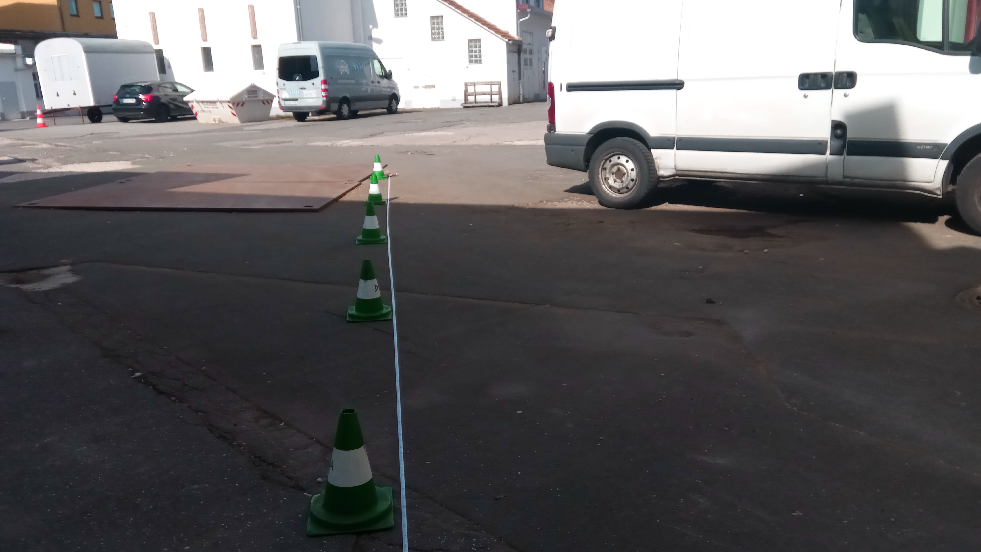
\includegraphics[width=0.5\textwidth]{Abb/start.png}
		\caption{example image}
		\label{example image}
	\end{figure}
	The picture is taken from a height of $1,2 m$ and the distance between the cones is $2m$ with the nearest $2m$ and the farthest $10m$ away from the camera. The resolution is 1920 by 1080 pixel. The resolution is chosen in a way that a CMOS camera can deliver 30 fps.
	 
	\subsection{Color Filtering}
	The most obvious feature is the color. So the first step is to implement a colorfilter. For this example it is obviously green but in the future a separate color-filter for blue, yellow and orange will be implemented.
	\begin{lstlisting}[language=Python]
hsv = cv2.cvtColor(image, cv2.COLOR_BGR2HSV)
	
# value for colorfilter
lower_green = np.array([30, 100, 0])
upper_green = np.array([90, 255, 255])
	
mask = cv2.inRange(hsv, lower_green, upper_green)
res = cv2.bitwise_and(hsv, hsv, mask=mask)

blur = cv2.GaussianBlur(res, (15, 15), 0)
return blur, mask
	\end{lstlisting}
	The image provided for the colorfilter needs to be converted from the RGB values to the HSV colorspace.
	The HSV describes the color not with an eight-Bit value for red, green and blue(RGB) but with a circle where the first value is for the color with 0 being red and 255 blue.
	The second value is needed for the saturation and the third describes how bright the color will be represented.
	
	With knowing how the HSV-colorspace works it is possible to find the right values which will describe the color of the cones. It will be necessary to try the colorfilter for images in bright sunlight as well as cloudy conditions to make sure to be able to detect cones in every possible environment.
	
	Next up is comparing every Pixel with our given value. With the OpenCV function "inRange" one image will be read and compared to the boundaries. It returns a binary image which means every pixel that was in range of the colorspectrum will be saved as a one/white and everything else will be a zero or black.
	
	\subsection{Contours}
	Searching for Contours on the black and white image is a easy task and delivers the same results every time.
	
	\begin{figure}[h]
		\centering
		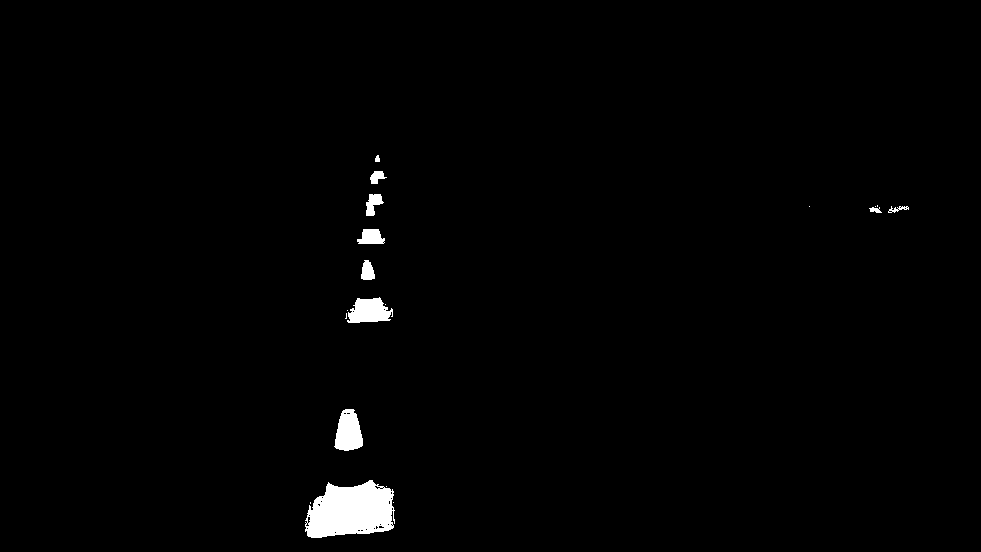
\includegraphics[width=0.5\textwidth]{Abb/mask.png}
		\caption{binary-image}
		\label{binary-image}
	\end{figure}
	
	But as seen in the top right hand corner of the image some noise will be left inside the picture. Depending on the scenery the colorfilter will always detect areas that are not of any interest. Therefore another filter is needed. A good difference between important and noisy areas, is the size of the contour. But you have to keep in mind, that deleting all small contours also deletes cones far away. The first test showed that excluding such cones does not matter.
	
	\subsection{Hierarchy}
	The color-filter left some pixel inside of the designated areas out and will show up as contours. Luckily the contour-function gives us back the hierarchy of each contour. By filtering out the parts lying inside of bigger areas leaves possible cone-areas with less noise.
	
	\subsection{Convex-Hull}
	Now only a handful of areas should be left, so executing intense operations on these contours will not make a big difference on the runtime of the code.
	The next step will be to find the convex hulls. A more precise description will be given in the section \ref{convex-hull}. The convex-hull leaves a very good approximation of the cones edges as seen in Figure \ref{convex-hull-picture}
	\begin{figure}[h]
		\centering
		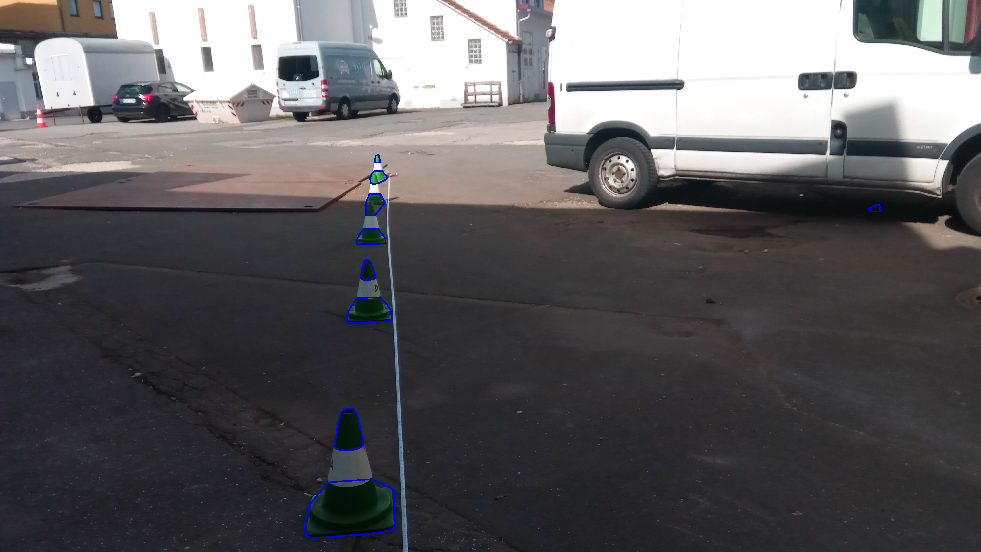
\includegraphics[width=0.5\textwidth]{Abb/convex-hull.png}
		\caption{convex-hull}
		\label{convex-hull-picture}
	\end{figure}
	
	\subsection{Aspect Ratio}
	A nice feature of the cones is the round top part. So no matter at what angle or distance the convex hull is detected the ratio between the height and width stays the same. With this Feature extracted, now all top parts of cones inside the image should be detected. As seen in the Figure \ref{top-part} it does not work perfectly as it does not track the ones standing behind each other. Knowing the Rules helps to estimate that this should be a rare occasion and two missed cones are better than a cone detected where there is none.
	\begin{figure}[h]
		\centering
		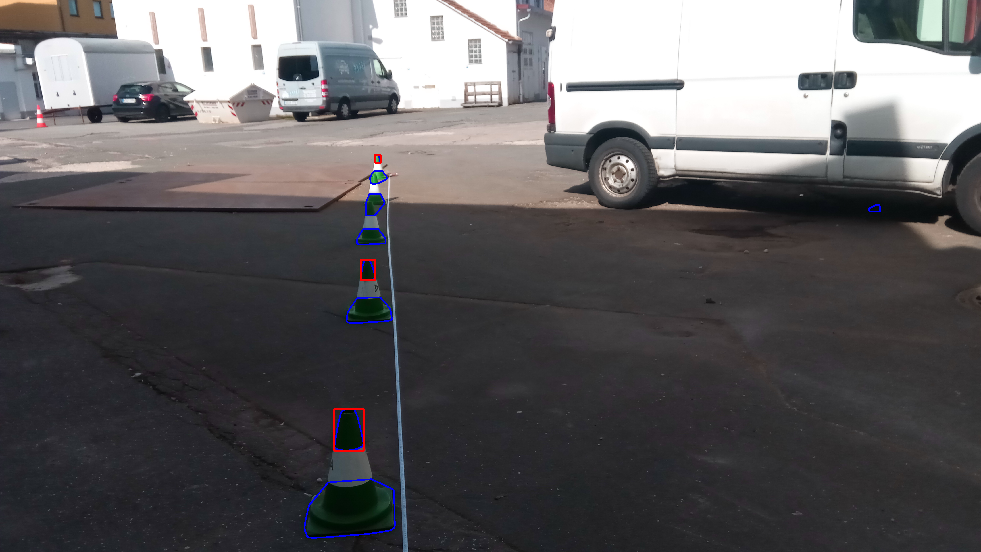
\includegraphics[width=0.5\textwidth]{Abb/top_part_cone.png}
		\caption{top-part}
		\label{top-part}
	\end{figure}
	
	
	\subsection{Bounding Box}
	With every top part of the cones found now the bottom part needs to be added. Therefore the distance to every other contour lying below is calculated and the nearest one belongs to the same cone.
	The maxima of both contours give the outlines of a bounding box which is drawn with red-color in Figure \ref{bounding-box}. This helps visualize what the computer detects and helps in further calculations for the distance estimation.
	
	\begin{figure}[h]
		\centering
		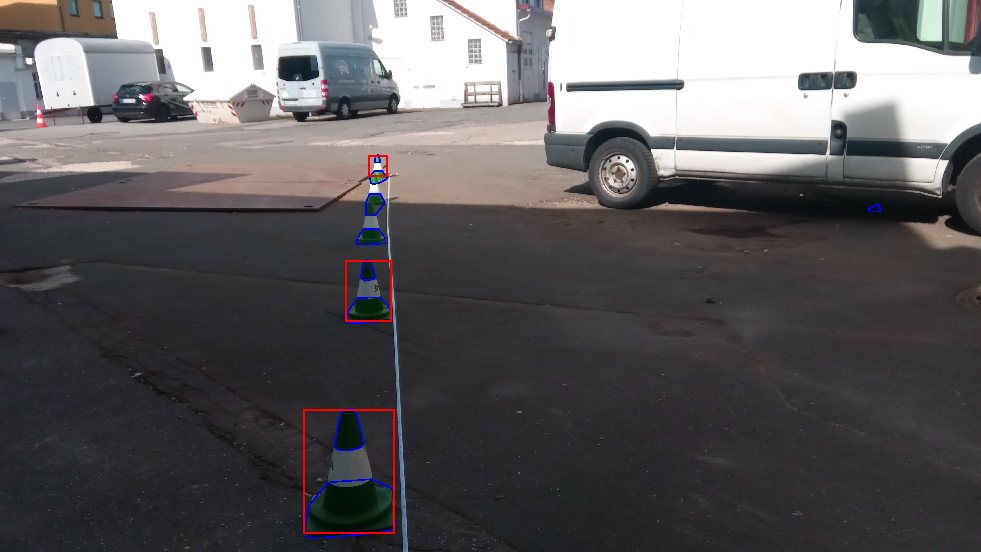
\includegraphics[width=0.5\textwidth]{Abb/bounding-box.png}
		\caption{bounding-box}
		\label{bounding-box}
	\end{figure}
	
	\section{Convex-Hull Algorithm by Graham and Yao} \label{convex-hull}
	The convex hull is a polygon with all points inside the boundaries while having no concave edges. Finding the Conex Hull is a well known problem with different solutions. OpenCV uses a gift-wrapping-algorithm introduced by Sklansky in 1982 \cite{opencv-doku} which is proved to be wrong on some special cases\cite{history-of-convex-hull}. To always find the right convex hull in a reasonable time an algorithm by Graham and Yao looks promising.
	
	
	
	\section{Distance Estimation}
	To find out where the cones are on the track the distance to each cone must be calculated. 
	With only one camera the number of pixel and a known height for a cone is the only value that can be used. It is also important to know the resolution of the used camera.
	While it is quite simple to take high-resolution pictures and then wait for a computer to analyze them, it is not so easy in a real-time application on mobile Hardware. To make sure the picture can be read and analyzed the input will be limited to an 1920x1080 px image which can be processed by a small computer-module like a Jetson-Nano with a frame-rate of about 30 fps.

	\subsection{Height} \label{height-estimation}
	% estimate the distance with the pixel in vertical direction 
	One possible feature is measuring the height by counting the pixel describing the y-Height($h$) of the detected cone. The bounding box function of OpenCV already gives back the number of pixels in the y-Direction. 
	\begin{figure}[h]
		\centering
		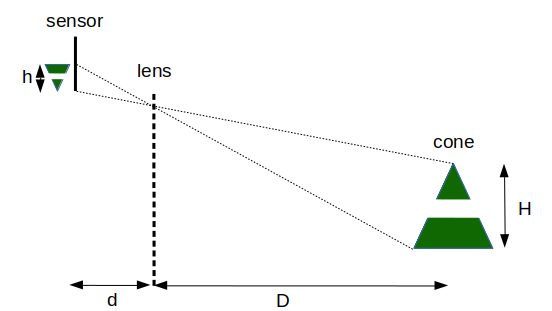
\includegraphics[width=0.5\textwidth]{Abb/distance-estimation.png}
		\caption{distance-estimation}
		\label{distance-estimation}
	\end{figure}
	The thin lens equation is given as
	$$\frac{D}{H}=\frac{d}{h}$$
	where $d$ is an unknown variable depending on the manufacturer of the camera.
	But $d$ can then be calculated with $d=\frac{D_1 \cdot h_1}{H}$ and then calibrated by taking a picture of a cone at a known distance. After evaluating the dimensions a good value is $D_1 \cdot h_1 = 440 \si{mpx}$.
	So to calculate the distance to each cone the following equation can be used:
	$$D = \frac{440}{h}$$
	
	\subsection{Width}
	Similar to the y-Dimension the bounding-Box-function gives back the x-Length. The math and algorithm for this distance estimation would be the same as for the height as it is for the error and possible disruption. Therefore it will not be discussed any further to make a clearer presentation.
	
	\subsection{Side-Length}
	% estimate distance with the distance between the top and bottom part of the cone
	The top part of a cone is round and so no matter at which angle the camera is detecting the cone, the proportions are the same. Being robust against rotation it is possibly a better feature for evaluating the distance.
	By using the side-length $s$ as described in Figure \ref{corners} for the distance estimation it can be valid for all angles of the cone.
	
	\begin{figure}[h]
		\centering
		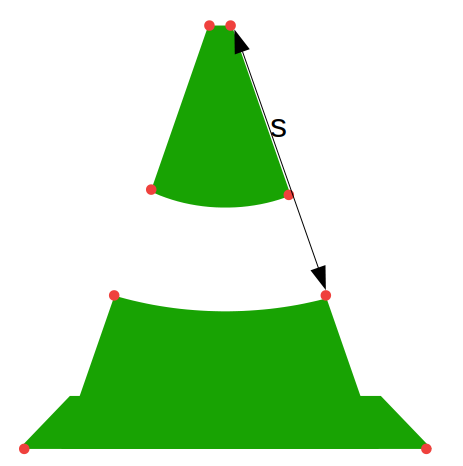
\includegraphics[width=0.3\textwidth]{Abb/corners.png}
		\caption{corners of a cone}
		\label{corners}
	\end{figure}
	
	To measure the side-length the corner points need to be found first. Inside of Figure \ref{corners} the important points are marked with red-dots.
	For all cases it can be estimated that the cone will have a flat point on the top and therefore both parts of the cone are trapezium-shaped.

	\begin{algorithm}
		\KwIn{convex-hull}
		\KwOut{extrem-points}
		find bounding Box\;
		get top-line\; 
		get bottom-line\;
		\While{point in convex hull}
			{\uIf{$y_{point} = y_{top-line}$}
				{\uIf{$x_{point} \le x_{left-top-corner}$}
					{left-top-corner = point;}
				\uIf{$x_{point} \ge x_{right-top-corner}$}
					{right-top-corner = point;}
				}
			\uIf{$y_{point} = y_{bottom-line}$}
				{\uIf{$x_{point} \le x_{left-bottom-corner}$}
					{left-bottom-corner = point;}
				\uIf{$x_{point} \ge x_{right-bottom-corner}$}
					{right-bottom-corner = point;}
			}
		}
	\label{extreme-points}
	\caption{extreme-points} 
	\end{algorithm}

	By drawing a bounding box around the contour the y-Dimension of the top and bottom corner-points can be estimated. Next step is to go through the points of the convex hull. If it lies inside a margin of the top or bottom line of the bounding boxes y-coordinates it is maybe a corner point. So the next step is then to look at the x-coordinates and compare if it lies more to the left or to the right then an already scanned point. That way the outermost points will be detected.
	
	The algorithm \ref{extreme-points} returns good corner points for cones standing upright. This code has to be run for the top section as well as the bottom section of the cone to be able to find all 8 corners.
	 
	By then calculating the distance between the Top-Right-corner of the top part to the Top-Right-corner of the bottom part the side-length of the cone can be calculated and used for a distance estimation similar to the one used in section \ref{height-estimation} with the calibrated value for $D_1 \cdot h_1 = 280 \si{mpx}$.
	$$D=\frac{280}{s}$$
	
	
	\subsection{Error}
	% estimate the error of the calculation
	With to much noise inside the image and low resolution the distance can not be accurate within a centimeter. But it is important to know how accurate each cone can be detected to know in which area a cone probably stands for the car to know how fast it can travel.
	
	\subsubsection{Rotation}
	One error can occur due to the angle the cone is facing the car. An example picture (Figure \ref{cone-rotated}) was taken to evaluate the  error by rotating one cone by 45�. 
	\begin{figure}[h]
		\centering
		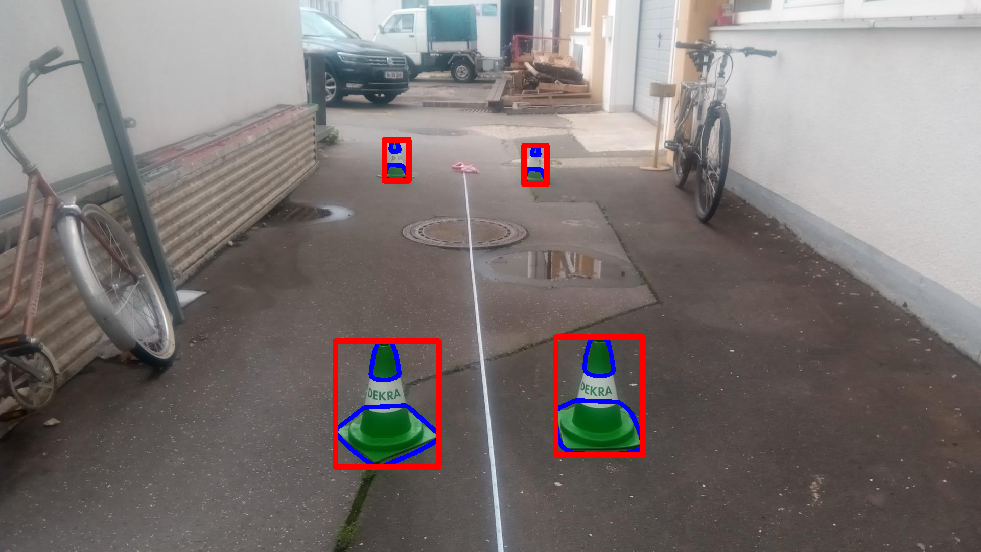
\includegraphics[width=0.7\textwidth]{Abb/cone-rotated.png}
		\caption{cone 45� rotated}
		\label{cone-rotated}
	\end{figure}
	The measurements for the cone $2m$ apart show a small difference with the estimation on the left side measuring $s_{45�} = 2,22m$ and $s_{0�} = 2,23m$ on the right side. So an overall difference between both measurements of just $\Delta_s = 0,01m$. The overall-height estimation gives back $s_{45�} = 1,79m$ and $s_{0�} = 1,90m$ with a delta of $\Delta_h = 0,11m$.
	For the cone $6m$ apart the error because of noise is already more important than the error occurred due to the rotation. Nevertheless the relative distance with $\Delta_s = 0,30m$ and $\Delta_h = 0,36m$ is still a little bit better.
	
	
	\subsubsection{Pixel-Error}
	To make sure the track can be monitored correctly it is important to know how good the distance estimation will be. By using only the number of pixels for an estimation you need to know how accurate the size can be estimated and how big the difference is for one pixel.
	$$\Delta D = \frac{\partial D}{\partial h} \cdot \Delta h = \frac{D_1 \cdot h_1}{h^2} \cdot \Delta h$$
	\begin{figure}[h]
		\centering
		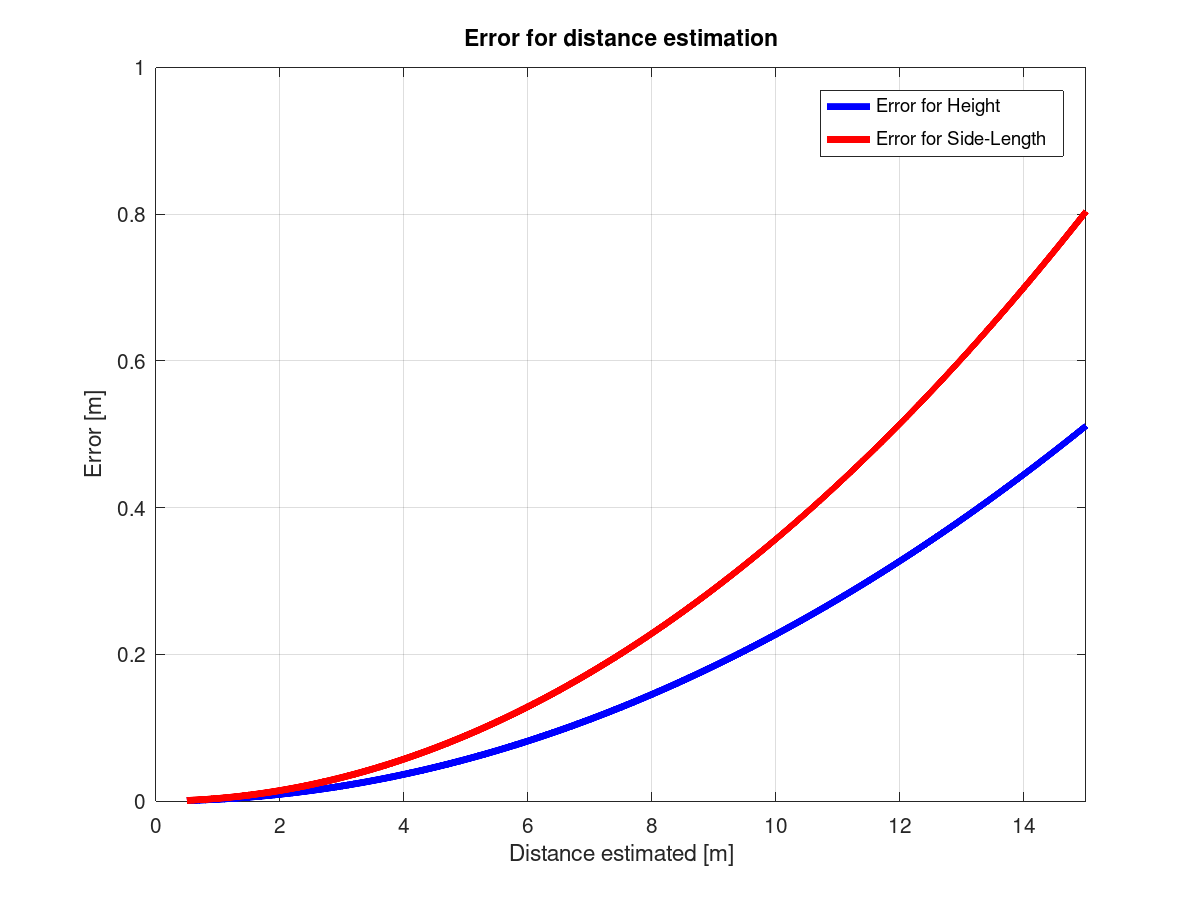
\includegraphics[width=0.7\textwidth]{Abb/pixel-error.png}
		\caption{error for one pixel}
		\label{error-pixel}
	\end{figure}
	
	\subsection{Disruption} \label{disruption}
	% discuss possible disruptions that can occur while driving (e.g bumps on the track)
	The most discouraging dial to get right will be the color-filter. It has to accurately detect the right color inside the image but it must not detect any yellow banners or the blue sky as cones, while working in bright sunlight as well as pouring rain.
	
	An often seen "DNF" (Did not Finish) in the driverless class is often detecting tipping over cones in one round and not being able to complete the track on the next round due to a imperfect course. So hopefully by detecting only the upstanding cones the ones not marking the true edge of the track wont disturb the car.
	
	\section{Tests}
	% test the algorithmus with different lighting and roadcondition
	An important test will be to what happens to a cone that is tipped over and lies somewhere on the track. Either it should not detected the cone at all or mark it as tipped over to ignore it for calculating its path.
	\begin{figure}[h]
		\centering
		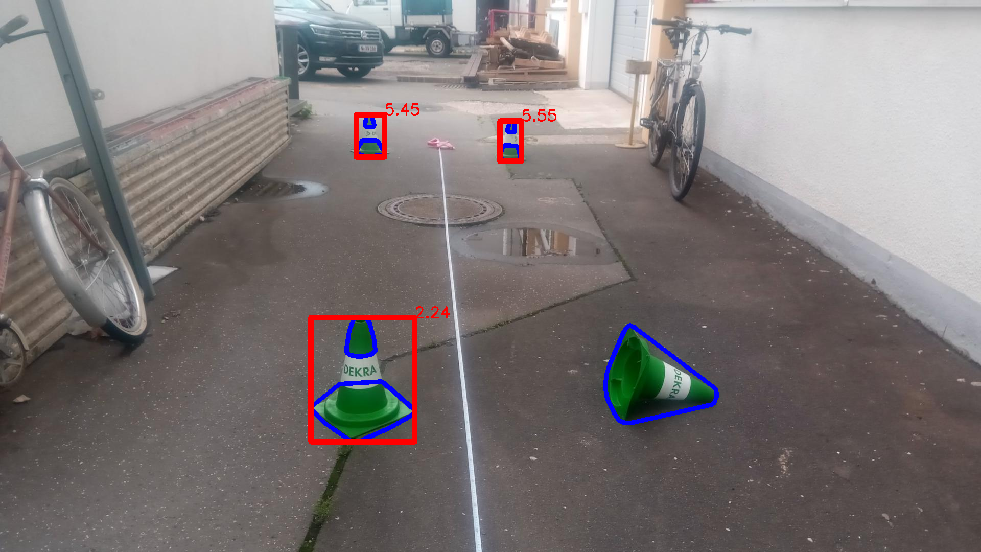
\includegraphics[width=0.5\textwidth]{Abb/cone-tipped.png}
		\caption{tipped cone}
		\label{cone-tipped}
	\end{figure}
	As seen in figure\ref{cone-tipped} the computer visualize a green area but does not detect it as a valid cone.
	
	Further tests can be done by using a computer generated image like done for Figure \ref{corners} and introducing possible disruption. They can be similar to the points discussed in section \ref{disruption} or be a marks (e.g. Dirt) on the cone in various sizes and forms.
	
	% \section{Summary}
	% after evaluating the tests
	
	\section{Discussion}
	% Steps in the future (e.g draw own pictures to test faulty inputs, test robustness of code)
	The best angle of the camera sill needs to be evaluated. For Testing purposes it was neglected but with cones coming closer to the car than $2m$ this can make a difference.
	
	
	Visualizing the cones for a computer algorithm works really good. Further tests to evaluate the robustness are needed, but with the distance estimation the next step towards creating a Map of the track can be taken. This is an important preprocess for a path-finding algorithms and to give the car the ability to know where on the track it is located. 
	It will be an exiting future with challenging and cool new projects for our Formula Student team.
	
	\begin{thebibliography}{}
		\bibitem{convex-hull}{Finding the Convex Hull of a Simple Polygon, Ronald L. Graham, F.Frances Yao, 1983}
		\bibitem{handbook}{FSG Competition Handbook 2020}
		\bibitem{opencv-doku}{OpenCV-docs(3.4.9).[Online] available on: https://docs.opencv.org/3.4.9/index.html. accessed on 08. July 2020}
		\bibitem{history-of-convex-hull}{G. Aloupis, A History of Linear-time Convex Hull Alorithms for Simple Polygons.[Online] available on: http://cgm.cs.mcgill.ca/~athens/cs601/. accessed on: 08. July 2020}
	\end{thebibliography}
\end{document}